\section{Proximal Policy Optimization (PPO)}
\label{sec:ppo}

% --- HOPPER RESULTS PLOT ---
\begin{figure*}[htbp]
    \centering
    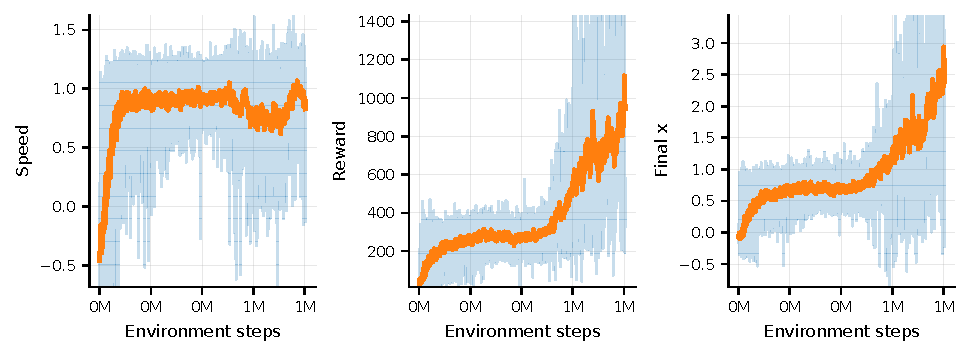
\includegraphics[width=\textwidth]{images/ppo_hopper_reward_speed_x.pdf}
    \caption{Training dynamics of PPO on the Hopper environment. (smoothed with an exponential moving average).}
    \label{fig:ppo_hopper_results}
\end{figure*}
% ---------------------------

\subsection{Algorithm Overview}

Proximal Policy Optimization (PPO)~\cite{schulman2017ppo} is an on-policy policy gradient method that directly optimizes a stochastic policy $\pi_\theta(a|s)$ by maximizing the expected discounted return. To prevent destructively large policy updates, PPO introduces a clipped surrogate objective:
\begin{equation}
    \mathcal{L}^{\text{CLIP}}(\theta) = \mathbb{E}_t \left[ \min\left( r_t(\theta)\hat{A}_t,\; \text{clip}(r_t(\theta), 1-\varepsilon, 1+\varepsilon)\hat{A}_t \right) \right],
\end{equation}
where $r_t(\theta) = \nicefrac{\pi_\theta(a_t|s_t)}{\pi_{\theta_\text{old}}(a_t|s_t)}$ is the probability ratio between the current and old policy, $\hat{A}_t$ is an estimate of the advantage function, and $\varepsilon$ is the clipping threshold. This formulation effectively constrains policy updates to a trust region without requiring computationally expensive second-order optimization.

PPO jointly optimizes a combined loss that also includes a value function term and an entropy bonus to encourage exploration:
\begin{equation}
    \mathcal{L}(\theta) = \mathcal{L}^{\text{CLIP}}(\theta) - c_1 \mathcal{L}^{\text{VF}}(\theta) + c_2 \mathcal{H}[\pi_\theta],
\end{equation}
where $c_1$ and $c_2$ are coefficients controlling the relative contribution of the value loss and the entropy bonus respectively. Advantages are estimated using Generalized Advantage Estimation (GAE)~\cite{schulman2018gae}, which balances bias and variance through a parameter $\lambda$:
\begin{equation}
    \hat{A}_t = \sum_{l=0}^{\infty} (\gamma\lambda)^l \delta_{t+l}, \quad \delta_t = r_t + \gamma V(s_{t+1}) - V(s_t).
\end{equation}

Unlike value-based algorithms like DQN, PPO operates natively in continuous action spaces by parameterizing the policy as a Gaussian distribution over actions. This makes it directly applicable to continuous control tasks without requiring any structural discretization or branching architectures.

\subsection{Hopper: Learning from Pixels}
\label{sec:ppo_hopper_results}

We first validate PPO on the Hopper task, maintaining identical environment and reward configurations to our previous value-based experiments to ensure a fair comparison.

\textbf{Configuration:}
The agent observes $64 \times 64$ pixel inputs with a frame stack of 4. We deploy 30 parallel environments to increase data throughput and stabilize advantage estimation, keeping the widened \texttt{healthy\_angle\_range} of $[-0.4, 0.4]$. The reward shaping remains focused on a target forward velocity of $1.5$ units/s ($w_{\text{vel}} = 1.0$), with a smoothness penalty ($w_{\text{ctrl}} = 0.001$) and a survival bonus ($w_{\text{healthy}} = 1.0$). PPO is trained for 1.5 million environment frames. Rollouts collect 256 steps per parallel environment before executing 10 epochs of minibatch updates. These architectural and environment parameters were kept fixed throughout training.
The remaining PPO-specific hyperparameters were selected via Optuna: a clipping threshold of $\varepsilon = 0.1$, a GAE parameter of $\lambda = 0.975$, and a discount factor of $\gamma = 0.995$. The policy and value networks share a convolutional encoder but maintain separate MLP heads, optimized via Adam with a learning rate of $4 \times 10^{-4}$.

\textbf{Results and Discussion:}
PPO demonstrates vastly superior sample efficiency compared to both BDQN and Rainbow. In less than 1.5 million steps, the agent successfully learns to chain multiple forward hops without falling, whereas standard DQN required tens of millions of frames ($\sim 40M$) to reach a similar milestone. Rainbow achieves similar results in the same number of frames, but training is much slower.

However, the learned behavior is functionally sub-optimal. The agent's step-wise velocity converges to approximately $1.0$ units/s, falling short of the $1.5$ target. Rather than developing the rapid, fluid momentum observed in our best Rainbow models (which naturally exceeded the target), PPO discovers a more conservative strategy. It fumbles slightly between jumps to deliberately regain its balance before committing to the next hop. While the upward trajectory of the learning curve suggests further velocity improvements are possible with longer training horizons, we also noted severe hyperparameter brittleness. Specifically, the target KL-divergence threshold was exceptionally difficult to tune, often leading to premature policy collapse if not perfectly calibrated.

\subsection{Humanoid: Scaling to High-Dimensional Control}
\label{sec:ppo_humanoid_results}

Following the Hopper experiments, we scaled PPO to the Humanoid environment. PPO theoretically avoids the combinatorial explosion that crippled standard DQN by directly outputting a continuous Gaussian policy over all 17 joint torques.

\textbf{Configuration:}
We applied the same morphological simplifications as our prior experiments, freezing the Z-axis rotations of the abdomen and hips, disabling the arms entirely, and increasing the observation resolution to $96 \times 96$ pixels. To tackle the extreme hyperparameter sensitivity observed in the Hopper task, we utilized Optuna to conduct extensive automated hyperparameter searches over the PPO training parameters. We relied on hundreds of short-horizon trials to rapidly prune diverging configurations. For consistency with the Rainbow evaluation, we kept the environment constraints and reward weights fixed ($w_{\text{vel}} = 3.0$ and $w_{\text{healthy}} = 1.0$).

\textbf{Results and Discussion:}
Despite PPO's native handling of continuous action spaces and the aggressive, automated search provided by Optuna, the agent failed to learn a stable bipedal gait. None of the attempted configurations managed to successfully balance and propel the Humanoid forward within the constrained trial bounds. 

This failure largely stems from the fixed reward weights. While freezing the reward parameters was necessary to establish a direct comparison with Rainbow, it artificially restricted the optimization landscape for PPO. Actor-critic methods are notoriously sensitive to reward scaling and relative incentive ratios. Allowing Optuna to jointly tune the reward formulation alongside the core algorithm parameters, combined with a larger computational budget for extended trial horizons, would likely be required to successfully isolate a stable locomotion policy for this environment.